\documentclass[/home/hernan/Documentos/Apuntes_mecanica_teorica/main.tex]{subfiles}
\graphicspath{{\subfix{images/}}}

\begin{document}
	\section{Vectores}\label{sec:vectores}


	Esto ya deberían saberlo y probablemente se actualice de último $: \left . \right)$

	\newpage
	\section{Mecánica Newtoniana para una partícula}\label{sec: N.particula }

	A continuación se expresará la mecánica de partículas de forma idealizada, donde no se presenta ningún tipo de fuerza disipativa en el sistema de interés.


	\subsection{Leyes de Newton}

	Las leyes de Newton tal y como se expresarán a continuación son unicamente válidas para sistemas de referencias \textbf{inerciales}, es decir, sistemas de referencia que no poseen ningun tipo de aceleración.

	\marginnote{Un estado de \textbf{equilibrio} se refiere a que el cuerpo o sistema de interés se encuentra movientodose con velocidad lineal constante (\textbf{equilibrio dinámico}) o se encuentra en reposo (\textbf{equilibrio estático}). \vspace{2cm}}

	\begin{definition}[\textbf{Primera Ley de Newton o  Ley de la Inercia}]
		Un cuerpo mantiene su estado de equilibrio a menos de que una fuerza neta lo perturbe. Dicho de otra forma, un cuerpo siempre mantendrá su estado de equilibrio a menos de que una fuerza neta llegue a afectarlo.
		\begin{equation}
			\sum \vec{F} = \vec{0}
			\label{eq: Nfirstlaw}
		\end{equation}
		
	\end{definition}

	
	\begin{definition}[\textbf{Segunda Ley de Newton}]
		Un cuerpo que experimenta una fuerza neta diferente de cero, tendrá como resultado un cambio en su momentum lineal.
		
		\begin{equation}
			\sum \vec{F} = \frac{d \vec{p}}{dt} = \dot{\vec{p}}
			\label{eq: NSecondlaw}
		\end{equation}
	\end{definition}


	\begin{marginfigure}
		\begin{figure}[H]
			\centering
			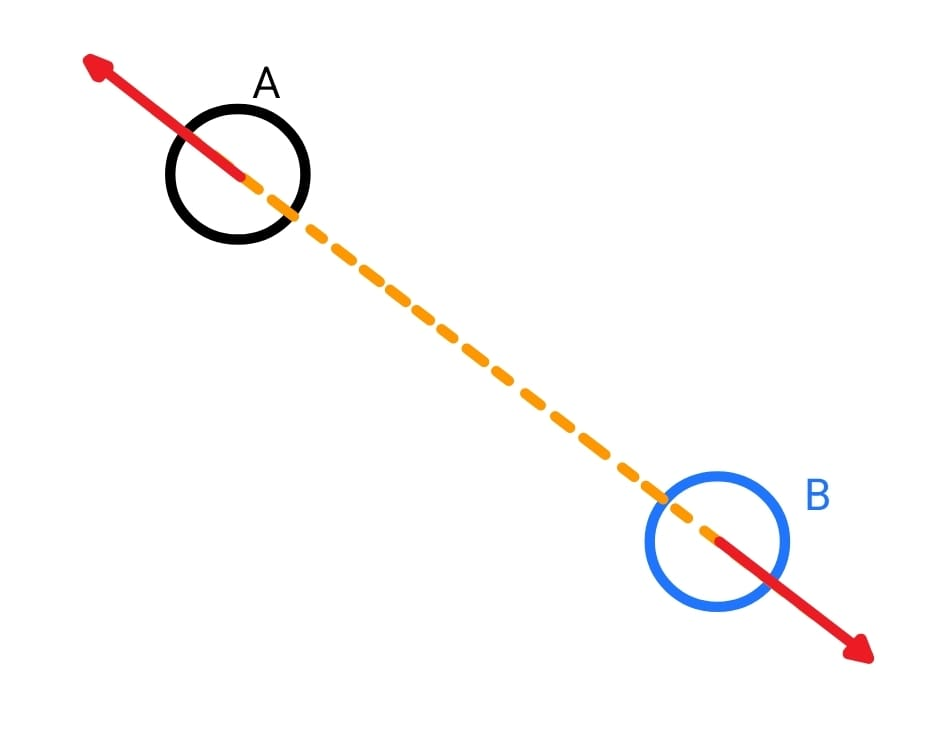
\includegraphics[width=4.5cm]{strongthirdlaw.jpeg}
			\caption{Situación del enunciado fuerte}
			\label{fig:Nthirdstrong}
		\end{figure}
	\end{marginfigure}

	\begin{marginfigure}
		\begin{figure}[H]
			\centering
			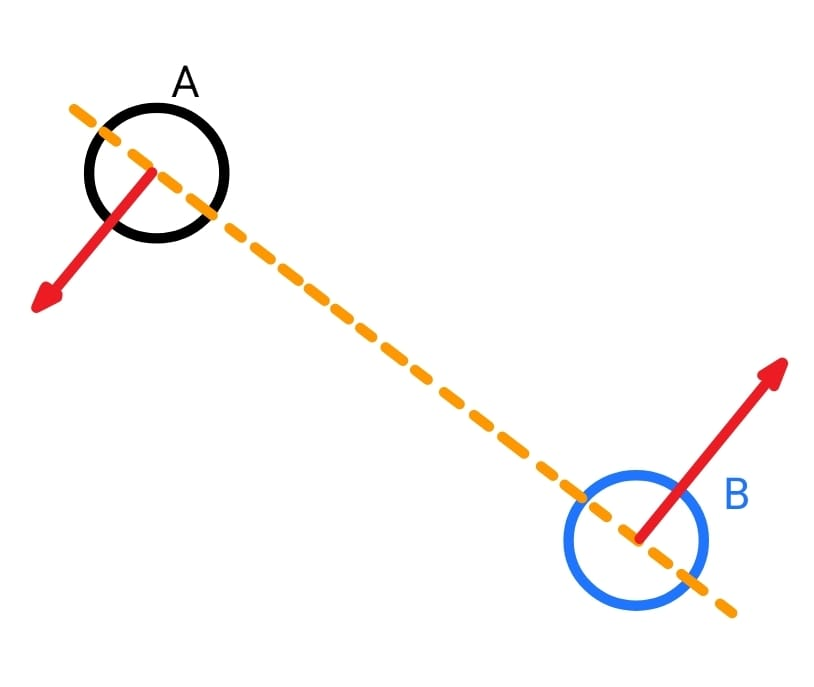
\includegraphics[width=4.5cm]{weakthirdlaw.jpeg}
			\caption{Situación del enunciado débil}
			\label{fig:Nthirdweak}
		\end{figure}
	\end{marginfigure}



	\begin{definition}[\textbf{Tercera Ley de Newton o Ley de Acción-Reacción}]
		Considere dos cuerpos denotados como A y B que presentan algún tipo de interacción entre sí, se dice que:
		Toda \textbf{acción} que realice el cuerpo A sobre el cuerpo B le corresponde una \textbf{reacción} que proveniente del cuerpo B. Estas \textbf{acciones} y \textbf{reacciones} corresponden a fuerzas internas del sistema (cuerpos A y B) debido a su interacción, dichas fuerzas poseen la misma magnitud y su dirección es contraria.
		
		\begin{equation}
			\vec{F}_{AB} = - \vec{F}_{BA}
			\label{eq: NThirdlaw}
		\end{equation}

		Para trabajar con esta ley hay que tomar cuenta cierta ambiguedad que nos lleva a los siguientes enunciados de la tercera ley:
		\begin{itemize}
			\item \textbf{Enunciado Fuerte: } Los vectores correspondientes a las fuerzas de \textbf{acción} y \textbf{reacción} se encuentran sobre una misma recta, es decir, sí se conocen las direcciones de las fuerzas de \textbf{acción} y \textbf{reacción} es posible trazar una recta (conocida como línea de acción) que una los vectores de fuerzas y sea paralela a estos.
			\item \textbf{Enunciado Débil: } No ocurre lo anterior. Es imposible unir los vectores de las fuerzas de \textbf{acción} y \textbf{reacción} por medio de una recta que sea paralela a ambos vectores.
		\end{itemize}
	\end{definition}
	\newpage

	\subsection{Trabajo y Energía}

	\begin{definition}[\textbf{Trabajo}] Corresponde a la cantidad generada al tomar el producto punto de la fuerza ejercida sobre un cuerpo a lo largo de todo su desplazamiento desplazamiento desde una punto A a un punto B.
		\begin{equation}
			W = \int_{A}^{B} \vec{F} \cdot d\vec{r}
			\label{eq: work}
		\end{equation}
	\end{definition}

	\begin{definition}[\textbf{Fuerza conservativa}] Una fuerza $\vec{F}$ es conservativa si se puede escribir de la forma:
		\begin{equation}
			\vec{F} = - \vec{\nabla}V
			\label{eq: conservativeforce}
		\end{equation}
	\end{definition}

	A partir de las ecuaciones \ref{eq: NSecondlaw} y \ref{eq: work}:

	\begin{align*}
		W & = \int_{A}^{B} \vec{F} \cdot d\vec{r} \; = \; \int_{A}^{B}  \frac{d \vec{p}}{dt} \cdot d\vec{r}
	\end{align*}

	Ejerciendo el producto punto y trabajando por índices:
	\begin{align*}
		W & = \int_{A}^{B} \sum_{i=1}^{3} \frac{d p_{i}}{dt}dr_{i}
	\end{align*}

	Suponiendo que la masa es constante, la derivada temporal del momentum lineal es de la forma: $\frac{d p_{i}}{dt} = m \frac{d v_{i}}{dt}$:

	\begin{align*}
		W & =  \sum_{i=1}^{3} m \int_{A}^{B} \frac{d v_{i}}{dt}dr_{i} =  \sum_{i=1}^{3} m \int_{A}^{B} \frac{d v_{i}}{dt}dr_{i} \frac{dt}{dt}\\ 
		& = \sum_{i=1}^{3} m \int_{A}^{B} d v_{i} \underbrace{\frac{d r_{i}}{dt}}_{= \: v_{i}} \cancelto{1}{\frac{dt}{dt}}\\
		& = \sum_{i=1}^{3} m \int_{A}^{B}  v_{i} d v_{i} = \left . \sum_{i=1}^{3} \frac{1}{2} m v_{i}^{2} \right|_{A} ^{B} = \sum_{i=1}^{3} \frac{1}{2} m v_{iB}^{2} - \sum_{i=1}^{3} \frac{1}{2} m v_{iA}^{2}
	\end{align*}

	\begin{definition}[\textbf{Energía Cinética}] Corresponde al trabajo necesario para comenzar a mover un cuerpo desde el reposo hasta la rapidez $\vec{v}$.

		\begin{equation} 
			T =  \frac{1}{2} m \sum_{i=1}^{3} v_{i}^{2}
			\label{eq:kineticenergy}
		\end{equation}
	\end{definition}

	\begin{theorem}[\textbf{Trabajo - Energía Cinética}]

		\begin{equation}
			W = \Delta T
			\label{eq: workT}
		\end{equation}
		
	\end{theorem}

	Regresando a la definición \ref{eq: work} pero ahora tomando la fuerza que es ejercida sobre el cuerpo como una fuerza conservativa, ecuación \ref{eq: conservativeforce}.

	\begin{align*}
		W &= \int_{A}^{B} \vec{F} \cdot d\vec{r} =  \int_{A}^{B} - \vec{\nabla}V \cdot d\vec{r} = -V_{B} + V_{A}
	\end{align*}

	\begin{definition}[\textbf{Energía Potencial}] Corresponde a la capacidad de un cuerpo de ejercer trabajo se denomina energía potencial. Ahora se presentan algunos ejemplos de energías potenciales.

		\begin{equation}
			V = \left \{ \begin{matrix}
				mgh\\ 
				\\
				\frac{1}{2}kx^{2} \\
				\\
				\frac{-GMm}{r}\\ 
				\\
				\frac{-Kq_{1}q_{2}}{r}\\ 
				\vdots 
				\end{matrix} \right .
		\end{equation}
		
	\end{definition}

	\begin{theorem}[\textbf{Trabajo - Energía Potencial}]

		\begin{equation}
			W = - \Delta V
			\label{eq: workV}
		\end{equation}
		
	\end{theorem}

	\subsection{Teoremas de Conservación}
	

\end{document}